%%%%%%%%%%%%%%%%%%%%%%%%%%%%%%%%%%%%%%%%%
% Masters/Doctoral Thesis 
% LaTeX Template
% Version 2.5 (27/8/17)
%
% This template was downloaded from:
% http://www.LaTeXTemplates.com
%
% Version 2.x major modifications by:
% Vel (vel@latextemplates.com)
%
% This template is based on a template by:
% Steve Gunn (http://users.ecs.soton.ac.uk/srg/softwaretools/document/templates/)
% Sunil Patel (http://www.sunilpatel.co.uk/thesis-template/)
%
% Template license:
% CC BY-NC-SA 3.0 (http://creativecommons.org/licenses/by-nc-sa/3.0/)
%
%%%%%%%%%%%%%%%%%%%%%%%%%%%%%%%%%%%%%%%%%

%----------------------------------------------------------------------------------------
%	PACKAGES AND OTHER DOCUMENT CONFIGURATIONS
%----------------------------------------------------------------------------------------

\documentclass[
11pt, % The default document font size, options: 10pt, 11pt, 12pt
oneside, % Two side (alternating margins) for binding by default, uncomment to switch to one side
english, % ngerman for German
singlespacing, % Single line spacing, alternatives: onehalfspacing or doublespacing
%draft, % Uncomment to enable draft mode (no pictures, no links, overfull hboxes indicated)
%nolistspacing, % If the document is onehalfspacing or doublespacing, uncomment this to set spacing in lists to single
%liststotoc, % Uncomment to add the list of figures/tables/etc to the table of contents
%toctotoc, % Uncomment to add the main table of contents to the table of contents
%parskip, % Uncomment to add space between paragraphs
%nohyperref, % Uncomment to not load the hyperref package
headsepline, % Uncomment to get a line under the header
%chapterinoneline, % Uncomment to place the chapter title next to the number on one line
%consistentlayout, % Uncomment to change the layout of the declaration, abstract and acknowledgements pages to match the default layout
]{MastersDoctoralThesis} % The class file specifying the document structure

\usepackage[utf8]{inputenc} % Required for inputting international characters
\usepackage[T1]{fontenc} % Output font encoding for international characters
\usepackage{listings} % for code chunks
\usepackage{enumitem,kantlipsum} % to indent paragraphs in enumerated lists

\usepackage{mathpazo} % Use the Palatino font by default

\usepackage[backend=bibtex,style=authoryear,natbib=true]{biblatex} % Use the bibtex backend with the authoryear citation style (which resembles APA)

\addbibresource{master-thesis-template.bib} % The filename of the bibliography

% for inserting images
\usepackage{graphicx}
\graphicspath{ {Images/} }

\usepackage[autostyle=true]{csquotes} % Required to generate language-dependent quotes in the bibliography

% for tables formatting
\usepackage{array}
\newcolumntype{X}{>{\centering\arraybackslash}m{4cm}}
\newcolumntype{L}{>{\centering\arraybackslash}m{3cm}}
\newcolumntype{M}{>{\centering\arraybackslash}m{2cm}}
\newcolumntype{T}{>{\centering\arraybackslash}m{1.5cm}}
\newcolumntype{S}{>{\centering\arraybackslash}m{1cm}}
\newcolumntype{N}{@{}m{0pt}@{}}
\usepackage{multirow}
\usepackage{fp,xcolor,colortbl}

% for equations 
\usepackage{amsmath}

% todo notes
\usepackage[colorinlistoftodos,prependcaption]{todonotes}

\newcommand{\he}[1]{%
    \FPeval{\resa}{max(0, 
    %min(1, 1-(#1-min_table_value)/(max_table_value-min_table_value)+adjustment))
    min(1, 1-(#1-58.8)/(88.2-58.8)+0.3))}%
    \edef\processme{\noexpand\cellcolor[gray]{\resa}}%
    \processme
    \FPiflt{\resa}{0.5}%
      \color{white}%
    \fi
    #1%
}

%----------------------------------------------------------------------------------------
%	MARGIN SETTINGS
%----------------------------------------------------------------------------------------

\geometry{
	paper=a4paper, % Change to letterpaper for US letter
	inner=2.5cm, % Inner margin
	outer=3.8cm, % Outer margin
	bindingoffset=.5cm, % Binding offset
	top=1.5cm, % Top margin
	bottom=1.5cm, % Bottom margin
	%showframe, % Uncomment to show how the type block is set on the page
}

%----------------------------------------------------------------------------------------
%	THESIS INFORMATION
%----------------------------------------------------------------------------------------

\thesistitle{Detection of Difficult for Understanding Medical Words using Deep Learning} % Your thesis title, this is used in the title and abstract, print it elsewhere with \ttitle
\supervisor{PhD. Artem \textsc{Chernodub}} % Your supervisor's name, this is used in the title page, print it elsewhere with \supname
\cosupervisor{PhD. Natalia \textsc{Grabar}}
\seccosupervisor{PhD. Thierry \textsc{Hamon}}
\examiner{} % Your examiner's name, this is not currently used anywhere in the template, print it elsewhere with \examname
\degree{Master of Science} % Your degree name, this is used in the title page and abstract, print it elsewhere with \degreename
\author{Hanna \textsc{Pylieva}} % Your name, this is used in the title page and abstract, print it elsewhere with \authorname
\addresses{} % Your address, this is not currently used anywhere in the template, print it elsewhere with \addressname

\subject{Data Science} % Your subject area, this is not currently used anywhere in the template, print it elsewhere with \subjectname
\keywords{} % Keywords for your thesis, this is not currently used anywhere in the template, print it elsewhere with \keywordnames
\university{\href{http://www.ucu.edu.ua}{Ukrainian Catholic University}} % Your university's name and URL, this is used in the title page and abstract, print it elsewhere with \univname
\department{\href{http://department.university.com}{Faculty of Applied Sciences}} % Your department's name and URL, this is used in the title page and abstract, print it elsewhere with \deptname
\group{\href{http://researchgroup.university.com}{Department of Computer Sciences}} % Your research group's name and URL, this is used in the title page, print it elsewhere with \groupname
\faculty{\href{http://faculty.university.com}{}} % Your faculty's name and URL, this is used in the title page and abstract, print it elsewhere with \facname

\AtBeginDocument{
\hypersetup{pdftitle=\ttitle} % Set the PDF's title to your title
\hypersetup{pdfauthor=\authorname} % Set the PDF's author to your name
\hypersetup{pdfkeywords=\keywordnames} % Set the PDF's keywords to your keywords
}

\begin{document}

\frontmatter % Use roman page numbering style (i, ii, iii, iv...) for the pre-content pages

\pagestyle{plain} % Default to the plain heading style until the thesis style is called for the body content

%----------------------------------------------------------------------------------------
%	TITLE PAGE
%----------------------------------------------------------------------------------------

\begin{titlepage}
\begin{center}

\vspace*{.06\textheight}
{\scshape\LARGE \univname\par}\vspace{1.5cm} % University name
\textsc{\Large Master Thesis}\\[0.5cm] % Thesis type

\HRule \\[0.4cm] % Horizontal line
{\huge \bfseries \ttitle\par}\vspace{0.4cm} % Thesis title
\HRule \\[1.5cm] % Horizontal line
 
\begin{minipage}[t]{0.4\textwidth}
\begin{flushleft} \large
\emph{Author:}\\
{\authorname} % Author name - remove the \href bracket to remove the link
\end{flushleft}
\end{minipage}
\begin{minipage}[t]{0.4\textwidth}
\begin{flushright} \large
\emph{Supervisor:} \\
{\supname} % Supervisor name - remove the \href bracket to remove the link
\vfill
\ \\
\emph{Co-supervisors:} \\
{\cosupname}\\
{\seccosupname}
\end{flushright}
\end{minipage}\\[1cm]
 
\vfill

\large \textit{A thesis submitted in fulfillment of the requirements\\ for the degree of \degreename}\\[0.3cm] % University requirement text
\textit{in the}\\[0.4cm]
\groupname\\\deptname\\[1cm] % Research group name and department name
 
\vfill

\includegraphics[height=5cm]{UCU-Apps.png} % University/department logo - uncomment to place it

\vfill
{\large Lviv 2019}\\[3cm] % Date
 
\vfill
\end{center}
\end{titlepage}

%----------------------------------------------------------------------------------------
%	DECLARATION PAGE
%----------------------------------------------------------------------------------------

\begin{declaration}
\addchaptertocentry{\authorshipname} % Add the declaration to the table of contents
\noindent I, \authorname, declare that this thesis titled, \enquote{\ttitle} and the work presented in it are my own. I confirm that:

\begin{itemize} 
\item This work was done wholly or mainly while in candidature for a research degree at this University.
\item Where any part of this thesis has previously been submitted for a degree or any other qualification at this University or any other institution, this has been clearly stated.
\item Where I have consulted the published work of others, this is always clearly attributed.
\item Where I have quoted from the work of others, the source is always given. With the exception of such quotations, this thesis is entirely my own work.
\item I have acknowledged all main sources of help.
\item Where the thesis is based on work done by myself jointly with others, I have made clear exactly what was done by others and what I have contributed myself.\\
\end{itemize}
 
\noindent Signed:\\
\rule[0.5em]{25em}{0.5pt} % This prints a line for the signature
 
\noindent Date:\\
\rule[0.5em]{25em}{0.5pt} % This prints a line to write the date
\end{declaration}

\cleardoublepage

%----------------------------------------------------------------------------------------
%	QUOTATION PAGE
%----------------------------------------------------------------------------------------

% \vspace*{0.2\textheight}

% \noindent\enquote{\itshape Thanks to my solid academic training, today I can write hundreds of words on virtually any topic without possessing a shred of information, which is how I got a good job in journalism.}\bigbreak

% \hfill Dave Barry

%----------------------------------------------------------------------------------------
%	ABSTRACT PAGE
%----------------------------------------------------------------------------------------

\begin{abstract}
\addchaptertocentry{\abstractname} % Add the abstract to the table of contents
In the medical domain, non-specialized users often require a better understanding of medical information provided by doctors. In this work, we address this need. We show how to improve identification of readability and understandability of medical words by applying novel embeddings received from RNN as features in the classification task. We also found out that adding pre-trained FastText word embeddings to the feature set significantly improves the performance of the classification model. For generalizability study of different models, we introduce a methodology comprising three cross-validation scenarios which allow testing classifiers in real-world conditions: when understanding of medical words by new users is unknown or when no information about understandability of new words is provided for the model.

\end{abstract}

%----------------------------------------------------------------------------------------
%	ACKNOWLEDGEMENTS
%----------------------------------------------------------------------------------------

\begin{acknowledgements}
\addchaptertocentry{\acknowledgementname} % Add the acknowledgements to the table of contents
First of all, I would like to thank my supervisor Artem Chernodub (Ukrainian Catholic University, Grammarly) who directed me throughout research for this thesis and provided a lot of useful pieces of advice regarding contents, structure and possible future development of the project. 

Also, I would like to thank Natalia Grabar (CNRS at Université de Lille, France), and Thierry Hamon (LIMSI, CNRS at Université Paris-Saclay, France and Université Paris 13, France) who agreed to proceed the work on detection of understandability of medical words, provided data for the research and actively participated in discussions on the project's progress and preparation of publications. 

Finally, I am grateful to Ukrainian Catholic University and Oleksii Molchanovskyi personally for the Master Program which was an important step in my career development as a data scientist. 

\end{acknowledgements}

%----------------------------------------------------------------------------------------
%	LIST OF CONTENTS/FIGURES/TABLES PAGES
%----------------------------------------------------------------------------------------

\tableofcontents % Prints the main table of contents

\listoffigures % Prints the list of figures

\listoftables % Prints the list of tables

%----------------------------------------------------------------------------------------
%	ABBREVIATIONS
%----------------------------------------------------------------------------------------

\begin{abbreviations}{ll} % Include a list of abbreviations (a table of two columns)

\textbf{NLP} & \textbf{N}atural \textbf{L}anguage \textbf{P}rocessing\\
\textbf{ANN} & \textbf{A}rtificial \textbf{N}eural \textbf{N}etwork\\
\textbf{DNN} & \textbf{D}eep \textbf{N}eural \textbf{N}etwork\\
\textbf{RNN} & \textbf{R}ecurrent \textbf{N}eural \textbf{N}etwork\\
\textbf{DT} & \textbf{D}ecision \textbf{T}ree\\
\textbf{CV} & \textbf{C}ross-\textbf{v}alidation\\
\textbf{GPU} & \textbf{G}raphics \textbf{P}rocessing \textbf{U}nit\\

\end{abbreviations}

%----------------------------------------------------------------------------------------
%	PHYSICAL CONSTANTS/OTHER DEFINITIONS
%----------------------------------------------------------------------------------------

% \begin{constants}{lr@{${}={}$}l} % The list of physical constants is a three column table

% The \SI{}{} command is provided by the siunitx package, see its documentation for instructions on how to use it

% Speed of Light & $c_{0}$ & \SI{2.99792458e8}{\meter\per\second} (exact)\\
%Constant Name & $Symbol$ & $Constant Value$ with units\\

% \end{constants}

%----------------------------------------------------------------------------------------
%	SYMBOLS
%----------------------------------------------------------------------------------------

\begin{symbols}{lll} % Include a list of Symbols (a three column table)

$A$ accuracy \\
$P$ precision \\ 
$R$ recall \\
$F$ F1 score \\
$\mu$ mean of a sample \\ 
$\sigma$ standard deviation of a sample \\
\todo{add symbols from formulas}
% $a$ & distance & \si{\meter} \\
% $P$ & power & \si{\watt} (\si{\joule\per\second}) \\
% %Symbol & Name & Unit \\

% \addlinespace % Gap to separate the Roman symbols from the Greek

% $\omega$ & angular frequency & \si{\radian} \\

\end{symbols}

%----------------------------------------------------------------------------------------
%	DEDICATION
%----------------------------------------------------------------------------------------

% \dedicatory{For/Dedicated to/To my\ldots} 

%----------------------------------------------------------------------------------------
%	THESIS CONTENT - CHAPTERS
%----------------------------------------------------------------------------------------

\mainmatter % Begin numeric (1,2,3...) page numbering

\pagestyle{thesis} % Return the page headers back to the "thesis" style

% Include the chapters of the thesis as separate files from the Chapters folder
% Uncomment the lines as you write the chapters

\chapter{Introduction}

\section{Motivation}
Specialized areas, such as medical area, convey and use technical words, or terms, which are typically related to knowledge developed within these areas. In the medical area, this specific knowledge often corresponds to fundamental medical notions related to disorders, procedures, treatments, human anatomy, etc. For instance, technical terms like \textit{blepharospasm} (abnormal contraction or twitch of the eyelid), \textit{alexithymia} (inability to identify and describe emotions in the self), \textit{appendicectomy} (surgical removal of the vermiform appendix from intestine), or \textit{lombalgia} (low back pain) are frequently used in the medical area texts.

As in any specialized areas, two main kinds of users exist in the medical area:

\begin{itemize}
    \item medical doctors, both researchers of practitioners, are experts of the domain. They contribute to the creation and development of biomedical knowledge and its exploitation for the healthcare process of patients;
    
    \item  patients and their relatives are consumers of the healthcare process. Usually, they do not have expert knowledge, while it is important that they understand the purpose and issues of their healthcare process. 
\end{itemize}
%%
If the understanding of technical medical terms is easy for the medical staff, patients and their relatives may present some difficulties in the understanding and using of such terms: they show indeed poor \textit{health literacy}. 

Hence, the existing literature provides several studies dedicated to the understanding of medical notions and terms by non-expert users, and on their impact on a successful healthcare process \citep{Mcgray-JAMIA2005,Eysenbach-JMIR2007}. Yet, it is not uncommon that patients and their relatives must face very technical health documents and information. Examples of this kind are frequent and usually the non-expert users are at loss in such situations:

\begin{itemize}
    \item  understanding of information on drug intake \citep{VanderStichele-WILEY1999,Patel-IJMI2002}, such as instructions related to the description and specification of steps necessary for the preparation and intake of drugs,
    
    \item  understanding of clinical documents \citep{Zeng-MEDINFO2007}, which contain important information on the healthcare process of patients,
    
    \item  understanding of clinical brochures or informed consents \citep{Williams-JAMA1995}, which are specifically created for patients and which are typically read by patients during their clinical pathway,
    
    \item  more generally, understanding of information provided for patients by different websites \citep{Oregon-2008,Brigo-EB2015} in different languages (English, Spanish, French) and different medical specialties,
    
    \item  for the same reasons, communication between patients and medical staff \citep{Jucks-HC2007,Tran-EC2009} remains complicated.
\end{itemize}
%%
These various observations provide the main motivation to our work. We propose to address the needs of non-specialized users in the medical domain. As we noticed, the main need is related to the understanding of medical and health information. 

\section{Thesis structure}
We first present some related work in chapter \ref{ch:related-work} and background knowledge in chapter \ref{ch:background-knowledge} which form the basis of the methods described in this work. We then introduce the data we used in chapter \ref{ch:dataset-description} and the proposed method in chapter \ref{ch:methodology}. Our results and their discussion are presented in Chapter 6. Finally, we conclude with some directions for future work in Chapter 7.

\chapter{Related Work}
\label{ch:related-work}

Related work is globally related to text simplification task which involves the detection of complex contents in documents and their adaptation for the target population. In this work we are interested in the first aspect with additional constraints: detection and diagnosis of technical contents in texts of medical domain. In general non-domain specific context, this task is also known in the literature as complex words identification (CWI). From the overview of related works it will be clear that in the NLP (Natural Language Processing) area, work related to the diagnosis of technical content in general and in medical domain in particular is quite frequent and topical. 

\section{Data sources for text understandability detection}

\todo[inline]{TH:I don't really understand why you make such distinction between NLP and Medical area: some (most of ?) works presented in the NLP section are related to the medical area, and  in medical area section, you mention some works related to NLP. There are in fact several mentioned points: (1) proposition of metrics (without considering NLP or Computer science approaches) for rating words according to their complexity for understanding (Flesch and Gunning); (2) design of resources or annotated texts, the purpose is to have reference for the evaluation or examples for ML approaches; (3a) word understanding and complexity in general language texts and (3b) in medical texts, both with NLP approaches. There is also another point to address: it is the reusability of the approaches on different languages (English, French), i.e. some approaches (Flesch for instance) have been developed for a Language (English) and it is a question to know if those approaches are relevant and useful for other languages (e.g. French) or not. I think also a last point to mention (here or in conclusion): here it is assumed that people who read the texts don't have problems or disabilities related to reading (e.g. dyslexia).  If you have time, it would good to reorganise the chapter, and may be mentioned limitations or additional aspects.}

% \todo{ngr: I would move the 1st paragraph to the previous section and name this section smth like "Suitable data for readability diagnosis"} - done

In detection of difficult for understanding contents a separate issue is to get suitable data for the analysis. These data have indeed crucial impact on models created and on their usability. Several approaches have been proposed:
\begin{itemize}
\item exploitation of expert judgment, who have an idea on needs of population aimed in the study \citep{DeClerc-NLE2014}. The main limitation is that experts may have difficulties to figure out what are the real needs of population;
\item exploitation of text books created for population according to their readability levels, such as school books \citep{Gala-ELEX2013}. The main limitation is that such books are
  usually created by experts using theoretical basis and observations;
\item exploitation of crowdsourcing involving large population \citep{DeClerc-NLE2014}.  The main limitation is that the population involved is uncontrolled and unknown;
\item exploitation of eye-tracking methods for a more fine-grained
  analysis of reading difficulties \citep{Yaneva-CCA2015,Grabar-ICHI2018}.  The main limitation is that only short text spans can be used;
\item manual annotation by human annotators \citep{Grabar-LREC2016t}. In this case, the annotators represent the population, they are part of the controlled population, they can
  perform more complicated tasks than in case of crowdsourcing, although they are usually less many than in crowdsourcing experiments. In this work the data source was constructed using this method. It also was expluatated in CWI challenges mentioned in the next section (SemEval-2016 and CWI 2018 Shared Task).
\end{itemize}
%%
Related to this issue is the question on generalizability of data and of models generated from these data.  For instance, it has been observed that data from experts are difficult to generalize over the population \citep{DeClerc-NLE2014}.


\section{Readability measures}
Readability provides a set of methods to compute and quantify the understandability of
words
Traditionally, researchers exploit the readability measures. Among these measures, it is possible to distinguish standard readability measures and computational readability measures \citep{Francois-TAL2013}. Classical measures usually rely on the number of letters and/or of syllables a word contains and on linear regression models \citep{Flesch1948,Gunning1973}, while computational readability
measures may involve vector models and great variability of
features, among which the following have been used for processing the
biomedical documents: a combination of classical readability formulas
with medical terminologies \citep{Kokkinakis-2006}; n-grams of
characters \citep{Poprat-MIE2006}, stylistic \citep{Grabar-AMIA2007} or
discursive \citep{Goeuriot-LREC2008} features, lexicon
\citep{Miller-HICSS2007}, morphological features
\citep{Chmielik-TAL2011}, combinations of different features
\citep{Zeng-MEDINFO2007}. At a more fine-grained level, the readability of words has been
addressed much less frequently. 

For general language, research actions are often performed as part of the NLP challenges. For the case pf CWI for example, there was a shared task on CWI on SemEval-2016 NLP challenge\footnote{\url{http://alt.qcri.org/semeval2016/task11/}}. The goal was to provide a framework for the evaluation of CWI methods, which involved:
\begin{enumerate}
    \item understanding the distinctive characteristics of words which are difficult for non-native speakers;
    \item finding out how well the vocabulary limitations of an individual can be predicted from the knowledge of vocabulary limitations of the group they are part of;
    \item introducing a gold-standard dataset for text simplification and tasks related to topic modeling and semantics.
\end{enumerate}

The participants applied rule-based and/or
machine learning systems, including neural networks for building solutions.
Combinations of various features, designed
to detect the complexity of words, have been used. The most popular among them were: 

\begin{itemize}
    \item simple features: word length, number of syllables, named-entity type, part-of-speech, position of word in sentence \citep{Bingel-SemEval2016};
    
    \item number of synsets, senses, synonyms, hyponyms, relations, distinct POSs in WordNet \citep{Ronzano-SemEval2016};
    
    \item corpus-based frequency in large corpora: Wikipedia, Simple Wikipedia \citep{Kauchak-2013}, SubIMDB \citep{Paetzold-SemEval2016solution}, British National Corpus \citep{Ronzano-SemEval2016}, Gigaword corpus and the International Conference on Web and Social Media (ICWSM) blog corpus \citep{Brooke-SemEval2016}. Mostly the frequency was calculated for word-level, but some participants utilized the frequency of char-level n-grams also \citep{Bingel-SemEval2016}.
\end{itemize}

The results of this shared task are described in detail in \cite{Paetzold-SemEval2016overview}. The analysis of 42 submitted systems by 21 teams highlighted that the most effectively CWI task is solved by decision trees \citep{Malmasi-SemEval2016} and ensemble methods \citep{Paetzold-SemEval2016solution, Ronzano-SemEval2016}. Moreover, according to the results, word frequencies remained the most reliable predicting feature of word complexity. The best systems reached up to 0.774 G-score, which measures the harmonic mean between Accuracy and Recall, and 0.353 F-score. 

In this challenge, attempts to apply neural networks showed poor results. Whereas after post-task experiments authors gained competitive results changing the framework of NN implementation, revising architecture and the feature set \citep{Bingel-SemEval2016}. Among features, 300-dimensional GloVe\footnote{\url{https://nlp.stanford.edu/projects/glove/}} word embeddings were found to be the main contributor to NN's performance improvement (from 0.506 to 0.756 G-score). 

Our task is slightly different from the one described in SemEval-2016 Shared task \citep{Paetzold-SemEval2016overview} where given a sentence and a target word within it, the goal is to predict whether or not a non-native English speaker would be able to understand the meaning of the target word. In our formulation we do not have the context near target medical words, so we cannot use it during the training. In other words, the task in SemEval-2016 is CWI in its ordinary meaning, whereas in our case the task comes down to words' classification. The usefulness of standard word embeddings for our task is also not clear, therefore. Moreover, in SemEval-2016 and our task user annotations are made in different languages: English and French correspondingly, -  and have different goals.

After the success of SemEval-2016, the second CWI Shared task\footnote{\url{https://sites.google.com/view/cwisharedtask2018/}} was organized at Building Educational Applications workshop 2018\footnote{\url{http://www.cs.rochester.edu/~tetreaul/naacl-bea13.html}}. This time the data was provided on four languages: English, German, Spanish and French. Whereas, for French, only the test set was available and no French training data. English corpora were extended and involved three genres: news, Wikinews and Wikipedia data. For comparison, on SemEval-2016 the corpora were formed from only Simple Wikipedia data. In 2018 the aim of the CWI Shared
task was to identify challenging for non-native speakers words based on the annotations collected from both native and non-native speakers. 
The analysis \citep{Yimam-BEA2018} of 12 submitted systems and 11 system description papers from 30 teams shows that traditional feature engineering-based approaches (mostly involving words' length and frequency features) still perform better than neural network and word embedding-based approaches. Whereas this time much more participants used deep learning approach in their solutions. This resulted in significant improvement of performance in CWI task on monolingual English track: the top rank systems reached from 0.811 to 0.874 F-score for different English datasets. At the same time cross-lingual German, Spanish and French tracks resulted in slightly lower F-score: 0.745, 0.769 and 0.759 correspondingly. Nevertheless, cross-lingual results were considered highly promising. This was the most important finding of this shared task. 
Among deep learning solutions used for resolving the CWI 2018 Shared Task  there were:
\begin{itemize}
    \item application of Convolutional Neural Network (CNN) for the first time for CWI task \citep{Aroyehun-BEA2018}. The solution is based on 2D convolution and word-embedding representation of the target text fragment and its context. The CNN-based system did not show significant improvement in performance compared to an alternative system based in feature engineering and Tree Ensembles developed by the same team. 
    
    \item a DNN which was feed with both word-level and character-level embeddings \citep{DeHertog-ACL2018}. The word-level representations were trained by team on their own on COW-corpora\footnote{\url{https://corporafromtheweb.org/}} with gensimfootnote{\url{https://radimrehurek.com/gensim/}} implementation of word2vec model (described in the next chapter \ref{sec:word2vec}). The character-level embeddings were trained by the DNN itself when learning to classify words into complex and non-complex.
\end{itemize}

In contrast to the last solution, in this work, we test the performance of FastText (described in the next chapter \ref{sec:fasttext}), which is a word2vec's modification and captures not only distributional properties of words but also morphological ones, as this model is trained on subword instead of word level. And again, in  CWI 2018 Shared Task words were provided in context, which is different to our setting.

In the medical area, we can mention three experiments: manual rating
of medical words \citep{Zheng-AMIA2002}, automatic rating of medical
words on the basis of their presence in different vocabularies
\citep{Borst-MIE2008}, and exploitation of machine learning approach
with various features \citep{Grabar-PITR2014}. This last experiment
achieved up to 0.85 F-measure on individual annotations.


 
\chapter{Background Information}
\label{ch:background-information}


% \begin{itemize}
%     \item Classification problem, methods to solve: log regression, trees, deep learning
%     \item How to evaluate quality of classification problem (accuracy, precision, recall, F1)
%     \item Word embeddings
%     \item RNNs and how to get embeddings from them
% \end{itemize}

\section{Classification problem}
Classification is a supervised machine learning problem. Given a set of $n$ attributes (features),a set of $k$ classes and a set of $m$ labeled training instances $$\{(x_i,y_i);i=1,...,m\},$$ where $x_i$ is a feature vector and $y_i$  is a label, the task is to find such a rule, which predicts the class of any instance from the values of its attributes.

A lot of real world problems can be considered as a classification problem, for instance \citep{Ng-2012cs229}:
\begin{itemize}
    \item understanding whether a tumor is malignant or benign by its size,
    \item distinguishing spam and non-spam emails by the words they contain,
    \item identifying fraudulent transactions among normal ones using their metadata.
\end{itemize}
To handle those tasks a large toolkit of classification algorithms currently exist, among which the most commonly used groups are: 
\begin{itemize}
 \item linear classifiers,
 \item support vector machines,
 \item nearest neighbours,
 \item decision trees,
 \item artificial neural networks.
\end{itemize} 

We will concentrate on the last two.

\subsection{Decision trees}
Decision threes are used for regression as well as for classification. In decision trees a tree-like model of decisions is used to provide the required output on tree's leaves. An example of decision tree is shown on fig. \ref{fig:decision-tree} This model is built as a sequence of conditional control statements based on values of different features characterizing input observation. A decision tree is mostly learned using recursive binary splitting technique. In this process on each step an algorithm is aimed to find the best feature and splitting condition to finally come up with the shortest path to the final decision. When a feature set is big, then stopping conditions are put on the decision tree to prevent the model from overfitting. 

\begin{figure}[h]
    \centering
    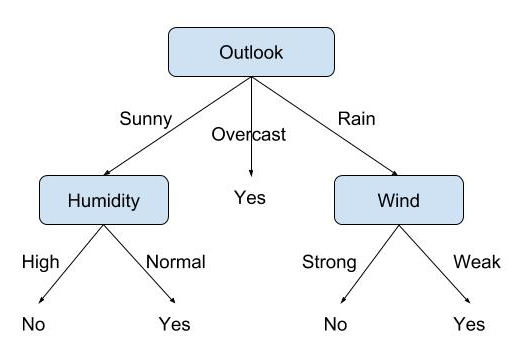
\includegraphics[width=8cm]{Images/Decision-tree.png}
    \caption{A decision tree for decision making about playing tennis on the day.}
    \label{fig:decision-tree}
\end{figure}
% \includegraphics[height=5cm]{Decision tree} 

The advantages of decision trees are:
\begin{itemize}
	\item simplicity of concept and interpretability,
	\item possibility to apply to both categorical and numeric data without a need of regularizaion. 
	\item easiness to combine with other decision techniques.
\end{itemize}

Disadvantages of decision threes are:
\begin{itemize}
	\item instability - a small change in data can lead to dramatic change in model,
	\item propensity of overfitting if no constraints are put.
\end{itemize}


\subsection{Artificial neural networks}
\todo{Do we need this section?}

\subsection{Classifier performance evaluation}

To evaluate a classifier the classification results are compared with class labels provided in training dataset. The experimental performance of a classifier on the test data is a proxy for the performance on unseen data. It checks the classifier’s generalization ability.
Binary classifiers are mostly evaluated using confusion matrix (fig. \ref{fig:confusion-matrix}).

\begin{figure}[h]
    \centering
    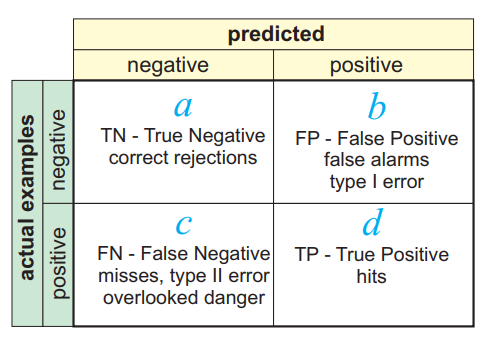
\includegraphics[width=8cm]{Images/Confusion-matrix.png}
    \caption{Confusion matrix. Source: \citep{kohavi:glossary}.}
    \label{fig:confusion-matrix}
\end{figure}

Performance measures calculated from the confusion matrix entries are the following:
\begin{itemize}
    \item Accuracy $= (a + d)/(a + b + c + d) =
    (TN + TP)/total$ ;
    \item True positive rate, recall, sensitivity$ =
    d/(c + d) = TP/actual\: positive$ ;
    \item Specificity, true negative rate $= a/(a + b) =
    TN/actual\: negative$ ; 
    \item Precision, predicted positive value $=
    d/(b + d) = TP/predicted\: positive$ ;
    \item False positive rate, false alarm $= b/(a + b)
    = FP/actual\: negative = 1 - specificity$ ;
    \item False negative rate $= c/(c + d) = FN/actual\: positive$ .
\end{itemize}

One of the measures above is not enough to evaluate a binary classifier properly when data in class imbalanced. For instance, on the examples on fig. \ref{fig:classifiers-evaluation} the accuracy is high and equal for both situations, but precision and recall are highly different. 


\begin{figure}[h]
    \centering
    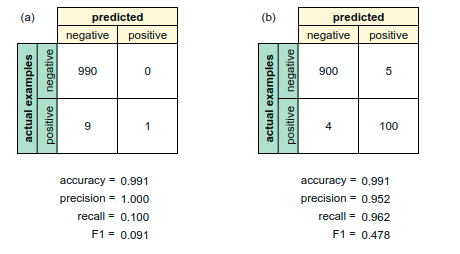
\includegraphics[height=8cm]{Images/Classifiers-evaluation.png}
    \caption{Examples of classifiers evaluation.}
    \label{fig:classifiers-evaluation}
\end{figure}

Moreover, it is always a question what to prioritize, precision or recall, and how to find balance among these two measures. For this reason, $F_1$ score, a harmonic mean of precision and recall, is frequently used to evaluate a binary classifier:

\begin{equation}
    F_{1}=2\cdot {\frac {\mathrm {precision} \cdot \mathrm {recall} }{\mathrm {precision} +\mathrm {recall} }}
\end{equation} 

\section{Vector words representations}

When working with textual data it is a popular approach in machine learning to represent words as vectors, which capture some relationships between words in language.

\subsection{Word2vec}
\todo[inline]{Reformulate next 3 paragraphs ( from  https://www.tensorflow.org/tutorials/representation/word2vec )}
Vector space models (VSMs) represent (embed) words in a continuous vector space where semantically similar words are mapped to nearby points ('are embedded nearby each other'). All methods in VSMs mostly rely on Distributional Hypothesis, which states that words that appear in the same contexts share semantic meaning. The approaches that leverage this principle can be divided into two categories:
\begin{itemize}
    \item count-based methods (e.g. Latent Semantic Analysis), where  the frequency of concurrence with neighboring words in a large text corpus is computed for each word, and then mapped onto a small, dense vector.
    \item predictive methods (e.g. neural probabilistic language models), where each word is predicted out of neighbours by means of learning small, dense embedding vectors, which are actually hidden layer values of a fully connected DNN. 
\end{itemize}

Word2vec is a computationally-efficient predictive model for learning word embeddings from raw text. It can be implemented using two approaches: Continuous Bag-of-Words model (CBOW) and  Skip-Gram model \cite{Mikolov-ICLR2013}. Both of this models are fully connected neural networks aimed to predict words, but CBOW predicts target words (e.g. 'mat') from source context words ('the cat sits on the'), while the skip-gram does the inverse and predicts source context-words from the target words. This inversion might seem like an arbitrary choice, but statistically it has the effect that CBOW smoothes over a lot of the distributional information (by treating an entire context as one observation). For the most part, this turns out to be a useful thing for smaller datasets. However, skip-gram treats each context-target pair as a new observation, and this tends to do better when we have larger datasets. 

A nice property of Word2vec words representation is that due to the way it is learned, final vectors capture context information of words. For this reason such vectors are frequently used as features for many canonical NLP prediction tasks, such as part-of-speech tagging, named entity recognition \citep{Collobert:DBLP}, or classification.


\subsection{Representations from RNN}
\todo{Not sure about the content of this section for now}
\chapter{Dataset description}
\label{ch:dataset-description}

For the experiments with the supervised words' categorization task in this work we used the publicly available set of words with annotations\footnote{\url{http://natalia.grabar.free.fr/resources.php\#rated}} collected according to the procedure described in \citep{Grabar-PITR2014}. Additionally, for the research of generalization abilities of our models described in \ref{sec:generalizability-study}, we were provided with four more sets of annotations.
The initial process of words' collection and annotation is briefly described below.

\section{Linguistic data description}
\label{sec:linguistic-data-description}

The set of required biomedical terms was obtained from the French part of Snomed International \citep{Cote-93} - a medical terminology\todo{th: I correct this point}, available from the ASIP SANTE website\footnote{\url{http://esante.gouv.fr/services/referentiels/referentiels-d-interoperabilite/snomed-35vf}}. The purpose of the terminology stored here is to provide an extensive up-to-date overview of the medical field. Snomed contains 151,104 medical terms organized into eleven semantic axes such as disorders and abnormalities, procedures, chemical products, living organisms, anatomy, social status, etc. For words' understandability study five axes related to the main medical notions were chosen: disorders, abnormalities, procedures, functions, and anatomy. These categories are assumed to contain terms which are familiar to a layman, in contrast to contents of such specific groups as chemical products (\textit{hydrogen sulfide}) and living organisms (\textit{Sapromyces, Acholeplasma laidlawii}).

The 104,649 selected terms were tokenized into words (or tokens) which are then lemmatized\todo{th: I made some modifications}, resulting in 29,641 unique words, for instance, the term `\textit{trisulfure d'hydrog\`{e}ne'} provided three words (\textit{trisulfure, de, hydrog\`{e}ne}).

\todo[inline]{th:you should indicate that the tokenization and the lemmatisation have been performed by TreeTagger \citep{Schmid-1994} and Flemm \citep{Namer-TAL2000}.}

The final dataset contains three morphological groups of words:
\begin{itemize}
    \item  compound words which contain several bases: abdominoplastie (abdominoplasty), dermabrasion (dermabrasion);
    \item  constructed words which contain one base and at least one affix: cardiaque (cardiac), acineux (acinic), lipo$\mathrm{\imath}$?de (lipoid);
    \item  simple words which contain one base, no affixes and possibly infections (when the lemmatization fails): acn\'{e} (acne), fragment (fragment).
\end{itemize}

\section{Annotation process}
\label{sec:annotation-process}
The set of 29,641 unique words was annotated by seven French speakers, 25-40-year-old, without medical training, without specific medical problems, but with the linguistic background. The annotators were expected to represent the average knowledge of medical words among the population as a whole. The annotators were presented with a list of terms and asked to assign each word to one of the three categories:

\begin{itemize}
    \item  I can understand the word;
    \item  I am not sure about the meaning of the word;
    \item  I cannot understand the word.
\end{itemize}
%%
The assumption is that the words, which are not understandable by the annotators, are also difficult to understand by patients. The annotators were asked not to use dictionaries during the annotation process. The annotation results are represented in Table \ref{tab:annot-results} .

\begin{table}[h]
\begin{tabular}{c|MMM|c}
\hline
\multicolumn{1}{l|}{\textit{Annotators / Categories}} & \textit{1. I can understand} & \textit{2. I am not sure} & \textit{3. I cannot understand} & \multicolumn{1}{M}{\textit{Total annotations}} \\ \hline
\textit{O1 (\%)} & 8,099 (28) & 1,895 (6) & 19,647 (66) & 29,641 \\
\textit{O2 (\%)} & 8,625 (29) & 1,062 (4) & 19,954 (67) & 29,641 \\
\textit{O3 (\%)} & 7,529 (25) & 1,431 (5) & 20,681 (70) & 29,641 \\
\textit{A1 (\%)} & 11,680 (39) & 2,312 (8) & 15,649 (53) & 29,641 \\
\textit{A2 (\%)} & 9,108 (31) & 2,994 (10) & 17,539 (59) & 29,641 \\
\textit{A7 (\%)} & 10,606 (36) & 2,206 (7) & 16,829 (57) & 29,641 \\
\textit{A8 (\%)} & 7,735 (26) & 1,032 (3) & 20,874 (70) & 29,641 \\ \hline
\end{tabular}
  \caption{Number (and percentage) of words assigned to reference categories by seven annotators (O1, O2, O3, A1, A2, A7, A8).}
    \label{tab:annot-results}
\end{table}


\todo[inline]{th: you should add a conclusion or a discussion, in order to conclude this chapter} 
\chapter{Methodology}
\label{ch:methodology}

The purpose of this work is to categorize medical words according to whether they can be understood or not by non-specialized people, using features obtained with deep learning methods. The manual annotations of these words described in the previous chapter provide the reference data. 

% The categorization pipeline is the following: after features for each word are computed, they are used for training the classifiers, and the results are evaluated using the cross-validation.

The proposed method includes three steps: 
\begin{enumerate}
    \item calculation of NLP features associated with the annotated words;
    \item training a machine learning model for words classification;
    \item evaluation of classification quality using cross-validation.
\end{enumerate}

In this research we want to provide answers to the following questions:
\begin{enumerate}
    \item Which feature set distinguishes better between understandable and non-understandable medical words?
    \item Why one feature set categorizes better than another?
    \item Do classifiers built on the considered feature sets generalize well? 
\end{enumerate}


\section{Feature sets}
\subsection{Standard NLP features}
\label{sec:standard-features}
We will refer to the previously used NLP features described in \citep{Grabar-PITR2014} as \textit{"standard features"} (opposed to two kinds of \textit{"embeddings"} described in the next subsection). The standard features include 24 linguistic and extra-linguistic features related to general and specialized languages. The features are computed automatically and can be grouped into ten classes: 

\begin{itemize}
\item {\it Syntactic categories.}  Syntactic categories and lemmas are
  computed by TreeTagger \citep{Schmid-1994} and then checked
  \todo{th: corrected} by Flemm
  \citep{Namer-TAL2000}.  The syntactic categories are assigned to
  words within the context of their terms.  If a given word receives
  more than one category, the most frequent one is kept as feature.
  Among the main categories we find for instance nouns, adjectives,
  proper names, verbs and abbreviations.
\item {\it Presence of words in reference lexica.} Two
  reference lexica of the French language were exploited:
  TLFi\footnote{\url{http://www.atilf.fr/}} and {\it lexique.org}\footnote{\url{http://www.lexique.org/}}. TLFi is
  a dictionary of the French language covering XIX and XX
  centuries. It contains almost 100,000 entries. {\it lexique.org} is
  a lexicon created for psycholinguistic experiments. It contains over
  135,000 entries, among which inflectional forms of verbs, adjectives
  and nouns. It contains almost 35,000 lemmas.
\item {\it Frequency of words through a non specialized search
    engine.} For each word, a query to Google search engine was sent in order to find out the frequency of the word attested on the web.
\item {\it Frequency of words in the medical terminology.} The frequency of words in the medical terminology Snomed International was computed.
\item {\it Number and types of semantic categories associated to
    words.} The information on the semantic categories of
  Snomed International was exploited.
\item {\it Length of words in number of their characters and
    syllables.} For each word, the number of its characters
  and syllables was computed.
\item {\it Number of bases and affixes.} Each lemma was analyzed by the
  morphological analyzer D\'erif \citep{Namer-AMIA2004}, adapted to the
  treatment of medical words. It performs the decomposition of lemmas
  into bases and affixes known in its database and it provides also
  semantic explanation of the analyzed lexemes. The
  morphological decomposition information (number of affixes and
  bases) was exploited.
\item {\it Initial and final substrings of the words.} Initial and final substrings of different length, from three to five characters, were computed.
\item {\it Number and percentage of consonants, vowels and other
    characters.} The number and the percentage of
  consonants, vowels and other characters (i.e., hyphen, apostrophe,
  comas) was computed.
\item {\it Classical readability scores.} Two classical
  readability measures were applied: Flesch \citep{Flesch1948} and its variant Flesch-Kincaid \citep{Kincaid-1975}. Such measures are typically used for evaluating the difficulty level of a text. They exploit surface
  characteristics of words (number of characters and/or syllables) and
  normalize these values with specifically designed coefficients.
\end{itemize}


\subsection{FastText word embeddings usage}

FastText word embeddings (described in section \ref{sec:fasttext}) is a good candidate as features for words difficulty detection task because they are able to use words' morphological information and generalize over it. The fact that word embeddings capture context and morphological information leads to the hypothesis that incorporating this information as features will improve classification accuracy for our specific problem. FastText embedding vectors are the sum of character n-gram representations, so that they could be generated even for unknown words. As we found out, being trained on Wikipedia and Common Crawl\footnote{\url{http://commoncrawl.org/}} texts the portion of known words from our dataset for current FastText embeddings is quite big. According to our analysis, 44.26\% (13,118 out of 29,641) medical words in the dataset and 56.00\% (16,598 out of 29,641) lowercased medical words in the dataset were used for training of the currently published FastText\footnote{\url{https://fasttext.cc}} model for French.

\subsection{French RNN Medical Understandability Text Embeddings (FrnnMUTE)}
\label{sec:frnnmute-learning}

According to the general functionality of RNN expressed in \ref{sec:rnn}, the final hidden state aggregates the information about all input sequence. This idea is frequently used to receive hidden representations of sequences. Sequence-to-sequence (seq2seq) models is a well-known example of how this idea works on practice \citep{Sutskever-NIPS2014}. Such models consist of two parts: an \textit{encoder} is an RNN which encodes input sequence into a representation in hidden space (which is also called \textit{thought vector}), and a \textit{decoder} which generates a new sequence out of the hidden representations (fig. \ref{fig:seq2seq}). 

\begin{figure}[h]
    \centering
    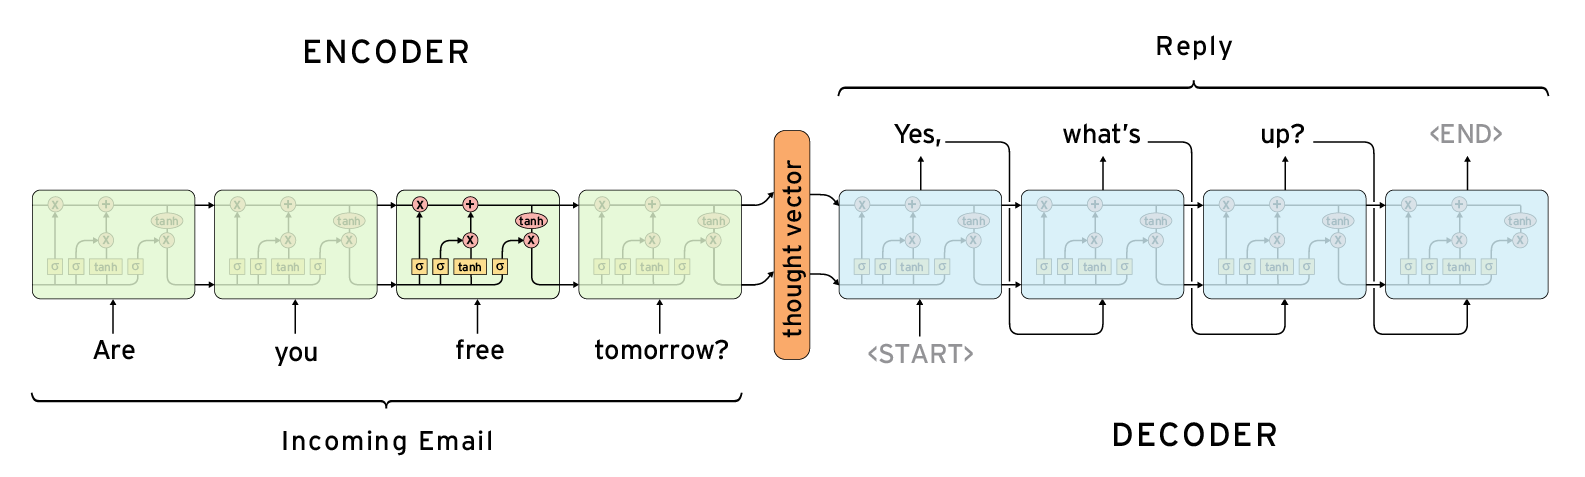
\includegraphics[width=14cm]{Images/seq2seq.png}
    \caption{A seq2seq model for question answering task. Source: \citep{Britz-2016}}
    \label{fig:seq2seq}
\end{figure} 

We utilized this idea for representing words from our dataset. To receive word representations from an RNN, we first trained it to classify words based on labels by one annotator (we chose $O1$), then for each word we found values of the last hidden state of the RNN and used this vector as features in words understandability detection for different users.

As a direct classifier, we trained a character-level RNN using PyTorch framework\footnote{\url{https://pytorch.org/}} and one GPU Tesla K80. For training we lowercased all words, converted them to a singular form and substituted all Unicode symbols with ASCII analogs.  We tried several RNN architectures and hyperparameter sets; the detailed information is available in Appendix \ref{appx:rnn}. 

The best F1-weighted on three classes we got for an RNN with to unidirectional Long short-term memory (LSTM) units (described in \ref{sec:lstm}), each with 50 hidden units. The dropout of the model is 0.7. The input size is 57 as the number of unique characters in lowercased and converted to ASCII input words. The output size is 3 as the number of classes in our data.

This model reached the best performance on the eighth epoch with $F1= 78.94$ and $accuracy = 81.21\%$ on development set. Using this model we received 50-dimensional words' representations which we called FrnnMUTE (French RNN Medical Understandability Text Embeddings). 


\section{Cross-validation scenarios}
For a thorough study of generalization abilities of the developed in this work classification models, we propose to consider three distinct cross-validation scenarios based on different combinations of users and vocabulary in train and test sets (fig. \ref{fig:experiments-description}).

\begin{figure}[h]
    \centering
    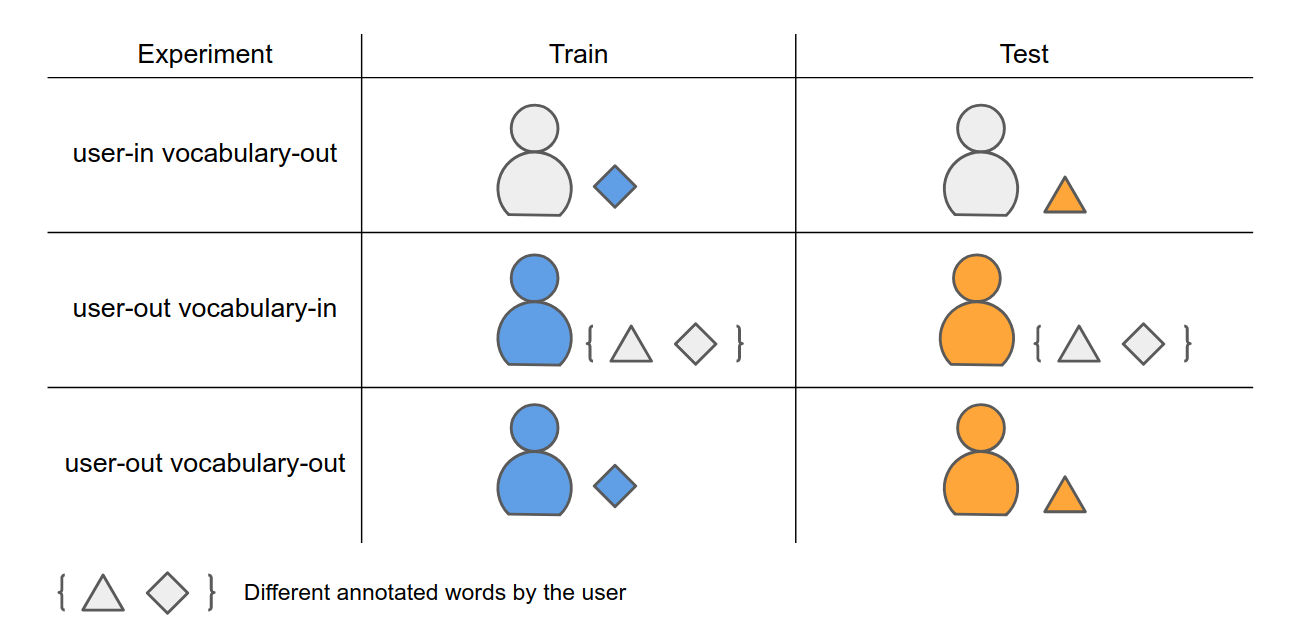
\includegraphics[width=14cm]{Images/Experiments.png}
    \caption{Visual description of experiments.}
    \label{fig:experiments-description}
\end{figure} 

\begin{enumerate}
    \item \textbf{User-in vocabulary-out cross-validation.} This type of experiment follows the scenario from the paper \citep{Grabar-PITR2014} we compare the results with throughout this work.  The cross-validation is done on each dataset (i.e., each user's annotation) separately. The goal of these experiments is to measure the ability of the method (classification model) to generalize class recognition on the \textit{known user} and his known manner to annotate words (that is, his understanding of the meaning of medical words) for \textit{unknown words}. 

\todo[inline]{In a pratical perspective: You may introduce the fact that user-in correspond to
  learning the profile of a user. So the model is a representation of
  the understanding/knowledge of the annotator.}
      
    \item \textbf{User-out vocabulary-in cross-validation.} In this experiment, we learn from all the annotations of one user and then test the model on annotations of another user. Thereby, in such a setting, we measure the ability of the classifier to generalize on all known words, but for unknown users. This scenario is realistic to a real-world situation: the reference annotations can be obtained only from a couple of users, presumably representing the overall population, but not from all the possible users. Yet, it is necessary to predict the familiarity of medical words for all the potential users even if they did not participate in the annotations.

\todo[inline]{similarly here, you can go further: The model represents the profile of a
  user/annotator and you try to identify if a new user has the same
  profile as a another. In that respect, for a user, the model that
  matches may be used to identify not understandable words for the new
user.}
      
    \item \textbf{User-out vocabulary-out cross-validation.} In this experiment, we take (k-1) folds of data from one user for training and use k-th fold for testing from the remaining user. In this case, we measure the ability of the method to generalize both on \textit{unknown users} and \textit{ unknown vocabulary}.

\todo[inline]{I think (but I'm not quite sure) that this last experiment must give you an idea of how many
  words you need to determine whether the profile of a user is the
  same as another.}
\end{enumerate}

\todo[inline]{You should add a conclusion or a discussion} 
\chapter{Experiments}
\label{ch:experiments}

\todo{Add trees depth for all tables}
We conducted a number of experiments to study the impact of adding vector words' representations as features to models on quality of classification. The quality of the applied classification algorithms was evaluated using four standard measures: accuracy $A$, precision $P$, recall $R$ and F1-measure $F$. These scores are weighted average for 1-vs-rest binary classifiers for each of three classes, described in \ref{sec:annotation-process}. Such evaluation of models allows to measure the ability of a chosen methodology (a feature set and a classification method) to distinguish understandable and non-understandable words in an unbalanced dataset. 

As in this work we compare results with ones in \cite{Grabar-PITR2014}, we first, reproduce results from the paper on the same datasets. Then check how FastText word embeddings influence the quality of classification in different cross-validation scenarios. We notice that in one scenario FastText word embeddings significantly and confidently improve performance of classification model, so the next step is to study whether this model generalized well on bigger variety of users. Finally, we study how RNN suprevised representations used as features impact on classification quality in all the same cross validation scenarios as preciously and on all available users.

\section{Reproduction of previous results}

In \citep{Grabar-PITR2014} the classification methods were obtained using WEKA \footnote{\url{https://www.cs.waikato.ac.nz/ml/weka/}} - a collection of machine learning algorithms for data mining tasks implemented on Java. In our research as a tool to conduct experiments we used Python, because it is easy to use and there are a lot of stable third-party Python libraries that make Python convenient for research. In order to ensure the consistency of experiments in this work and in \citep{Grabar-PITR2014}, firstly, we reproduced the WEKA results using pre-computed standard set of features from \citep{Grabar-PITR2014} and J48 classification algorithm based on Decision Tree (DT) - a WEKA implementation of C4.5 described in section \citep{Quinlan1993}. Our results perfectly match with ones presented in paper. Secondly, we developed a solution based on DT classifier from well-known scikit-learn library\footnote{\url{http://scikit-learn.org}}. At this step we got 0.85-1.41 lower $F$ scores for scikit-learn compared to WEKA results (Table \ref{tab:results-reproduction}).

\begin{table*}[h]
\begin{tabular}{L|LLL}
\hline
\textit{annotator \textbackslash method} & \textit{Results from paper \citep{Grabar-PITR2014}} & \textit{WEKA J48} & \textit{Python Decision trees (10-fold CV, with shuffle)} \\ \hline
$A1$ & 80.6 & 80.5 & 79.8 \\
$A2$ & 81.4 & 80.9 & 80.0 \\
$A3$ & 84.5 & 84.5 & 83.2 \\ \hline
\end{tabular}
    \caption{Comparison of various implementations for decision tree classifier on three datasets (A1, A2, A3) in user-in vocabulary-out cross-validation. The best score for a combination of quality measure and experiment among three feature sets is in bold.}
    \label{tab:results-reproduction}
\end{table*}

Since the input features were identical for WEKA and scikit-learn frameworks, we decided that this small degradation of quality is caused by the difference in implementations of decision tree classifiers in these frameworks. And so, in all subsequent experiments we will use the scikit-learn results reproduction because of it's convenience for comparison of experiments' results. 

% \section{Selection of classifier}
% Here will be shortly introduced results on using different classifiers and that DT was the best.

\section{Experiments with cross-validation settings}
\label{sec:cv-experiments}
\subsection{User-in vocabulary-out cross-validation}

These experiments also follow the scenario from \cite{Grabar-PITR2014}. The cross-validation is done on each dataset (i.e. each user's annotation) separately. The goal of these experiments is to measure the ability of the method to generalize class recognition on the \textit{known user} and his known manner to annotate words (that is, his understanding of the meaning of medical words) for \textit{unknown words}. 

We carried out the experiments using (i) the standard features only, (ii) the FastText word embeddings only and (iii) their combination. Experiments with isolated FastText ~word embeddings as features and the data from three annotators resulted in poor F-scores (Table \ref{tab:user-in-voc-out}), that can be treated that contextual information which is dominant in the word embeddings is not enough to define the word understandability. Adding the FastText word embeddings to the standard feature set resulted in up to 1\% higher F-score due to higher Precision (up to 1.8\%), meaning that contextual information slightly impacts on the understandability of a word by a given person.

\begin{table*}[h]
\begin{tabular}{cc|cccc|cccc|cccc}
\multirow{2}{0.6cm}{\textit{Train user}} & \multirow{2}{0.6cm}{\textit{Test user}} & \multicolumn{4}{c|}{\textit{Standard features only}} & \multicolumn{4}{c|}{\textit{Embeddings only}} & \multicolumn{4}{X}{\textit{Standard features + FastText word embeddings}} \\ \cline{3-14} 
 &  & $A$ & $P$ & $R$ & $F$ & $A$ & $P$ & $R$ & $F$ & $A$ & $P$ & $R$ & $F$ \\ \hline
$A1$ & $A1$ & \textbf{82.5} & 77.2 & \textbf{82.5} & 79.8 & 72.5 & 67 & 72.5 & 69.3 & 82.4 & \textbf{79} & 82.4 & \textbf{80.2} \\
$A2$ & $A2$ & \textbf{82} & 78.9 & \textbf{82} & 80 & 73.5 & 69.9 & 73.5 & 71.3 & 81.9 & \textbf{79.5} & 81.9 & \textbf{80.3} \\ 
$A3$ & $A3$ & 85.5 & 81.2 & 85.5 & 83.2 & 74.9 & 70.4 & 74.9 & 72.3 & \textbf{85.9} & \textbf{83} & \textbf{85.9} & \textbf{84.2} \\ \hline 
\end{tabular}
    \caption{Experiments on user-in vocabulary-out cross-validation}
    \label{tab:user-in-voc-out}
\end{table*}


\subsection{User-out vocabulary-in cross-validation}

In this experiment, we learn from all the annotations of one user and then test the model on annotations of another user. In this setting, we measure the ability of the classifier to generalize on all known words, but for unknown users (Table \ref{tab:user-out-voc-in}). This scenario is realistic to a real-world situation: the reference annotations can be obtained only from a couple of users, presumably representing the overall population, but not from all the possible users. Yet, it is necessary to predict the familiarity of medical words for all the potential users even if they
did not participate in the annotations.

\begin{table*}[h]
\begin{tabular}{cc|cccc|cccc|cccc}
\multirow{2}{0.6cm}{\textit{Train user}} & \multirow{2}{0.6cm}{\textit{Test user}} & \multicolumn{4}{c|}{\textit{Standard features only}} & \multicolumn{4}{c|}{\textit{Embeddings only}} & \multicolumn{4}{X}{\textit{Standard features + FastText word embeddings}} \\ \cline{3-14} 
 &  & $A$ & $P$ & $R$ & $F$ & $A$ & $P$ & $R$ & $F$ & $A$ & $P$ & $R$ & $F$ \\ \hline
\textit{A1} & \textit{A2} & 81.7 & 78.6 & 81.7 & 80.1 & 74 & 70.3 & 74 & 71.2 & \textbf{84.2} & \textbf{82} & \textbf{84.2} & \textbf{82.8} \\  
\textit{A1} & \textit{A3} & 85 & 81.2 & 85 & 83 & 75.4 & 70.7 & 75.4 & 72.6 & \textbf{87.6} & \textbf{84.9} & \textbf{87.6} & \textbf{85.9} \\ \hline 
\textit{A2} & \textit{A1} & 82.2 & 77 & 82.2 & 79.1 & 72.8 & 67.3 & 72.8 & 69.6 & \textbf{83.9} & \textbf{80.2} & \textbf{83.9} & \textbf{81.1} \\  
\textit{A2} & \textit{A3} & 85.4 & 81.1 & 85.4 & 83 & 75.3 & 71.1 & 75.3 & 73 & \textbf{86.8} & \textbf{83.5} & \textbf{86.8} & \textbf{84.7} \\ \hline 
\textit{A3} & \textit{A1} & 82.8 & 77.4 & 82.8 & 79.7 & 72.7 & 67.1 & 72.7 & 69.4 & \textbf{84.9} & \textbf{81.3} & \textbf{84.9} & \textbf{82.4} \\  
\textit{A3} & \textit{A2} & 82.2 & 79 & 82.2 & 80.2 & 74.1 & 70.4 & 74.1 & 71.6 & \textbf{84.2} & \textbf{82.1} & \textbf{84.2} & \textbf{82.8} \\ \hline 
\end{tabular}
    \caption{Experiments on user-out vocabulary-in cross-validation}
    \label{tab:user-out-voc-in}
\end{table*}


In these experiments we got a significant improvement of combined features in comparison to the standard features. When knowledge of words understandability of one user is used to predict it for another user, adding the FastText word embeddings provides up to 2.9 better F-score. Notice that used separately, standard features and embeddings shows similar performance as in user-in vocabulary-out cross-validation (Table \ref{tab:user-out-voc-in}). Our hypothesis is that there exists a robust nonlinear dependency between some subsets of standard features and subword-level components of FastText word embeddings. Testing this hypothesis is the topic of our further research.

\subsection{User-out vocabulary-out cross-validation}

In this experiment, we take (k-1) folds of data from one user for training and use k-th fold for testing from the remaining user. In this case, we measure the ability of the method to generalize both on \textit{unknown users} and \textit{ unknown vocabulary}.

The cross-validation setting is now the most strict and knowledge of words understandability of one user is used to predict whether another user will understand other medical words. In these experiments, embeddings provide approximately 0.5\% higher F-score in case of learning on users A1 and A3 (Table \ref{tab:user-out-voc-out}). When learning on user A2, embeddings decrease F by 0.5, which means that annotations and health literacy of user A2 are different from users A1 and A3. It seems that adding embeddings makes overfitting of machine learning model to the dataset. As a result, tests on other ``kind of word understandability'' and on combined features are less successful compared to using standard features only for learning. This may be due to the lack of systematicity in annotations of A2.

\begin{table*}[h]
\begin{tabular}{cc|cccc|cccc|cccc}
\multirow{2}{0.6cm}{\textit{Train user}} & \multirow{2}{0.6cm}{\textit{Test user}} & \multicolumn{4}{c|}{\textit{Standard features only}} & \multicolumn{4}{c|}{\textit{Embeddings only}} & \multicolumn{4}{X}{\textit{Standard features + FastText word embeddings}} \\ \cline{3-14} 
 &  & $A$ & $P$ & $R$ & $F$ & $A$ & $P$ & $R$ & $F$ & $A$ & $P$ & $R$ & $F$ \\ \hline
\textit{A1} & \textit{A2} & 81.7 & 78.6 & 81.7 & 80.1 & 73.6 & 69.9 & 73.6 & 71.3 & \textbf{81.8} & \textbf{79.8} & \textbf{81.8} & \textbf{80.6} \\ 
\textit{A1} & \textit{A3} & \textbf{85} & 81.2 & \textbf{85} & 83 & 74.8 & 70.4 & 74.8 & 72.4 & 84.9 & \textbf{82.2} & 84.9 & \textbf{83.4} \\ \hline 
\textit{A2} & \textit{A1} & \textbf{82.2} & 76.9 & \textbf{82.2} & \textbf{79.1} & 72.5 & 66.9 & 72.5 & 69.3 & 81.7 & \textbf{77.5} & 81.7 & \textbf{79.1} \\
\textit{A2} & \textit{A3} & \textbf{85.3} & 81 & \textbf{85.3} & \textbf{83} & 75.1 & 70.7 & 75.1 & 72.7 & 84.4 & \textbf{81.3} & 84.4 & 82.5 \\ \hline 
\textit{A3} & \textit{A2} & \textbf{82.7} & 77.3 & \textbf{82.7} & 79.7 & 72.5 & 66.9 & 72.5 & 69.2 & 82.6 & \textbf{78.9} & 82.6 & \textbf{80.2} \\ 
\textit{A3} & \textit{A3} & 82.1 & 79 & 82.1 & 80.1 & 73.8 & 70.2 & 73.8 & 71.4 & \textbf{82.2} & \textbf{80} & \textbf{82.2} & \textbf{80.7} \\ \hline 
\end{tabular}
    \caption{Experiments on user-out vocabulary-out cross-validation}
    \label{tab:user-out-voc-out}
\end{table*}

\section{Generalizability study}
\label{sec:generalizability-study}
In the previous experiments we concentrated on three annotators' data to be consistent with the research in paper \citep{Grabar-PITR2014}. To study better generalizability of models for words' understandability detection we included 4 more annotators in an experiment.

In this part we concentrated on the user-out vocabulary-in cross-validation scenario as the most realistic one. Here understanding of generalizability quality is crucial for usage of the model in real world client-doctor relationship.

\begin{table*}
  \centering
  \begin{tabular}{c|c|c|c|c||c|c|c||c|c|c}
    \it Train & \it Test  & \multicolumn{3}{c||}{\it Standard features} & \multicolumn{3}{c||}{\it Embeddings} & \multicolumn{3}{c}{\it Standard features}\\
    \it annotator & \it annotator & \multicolumn{3}{c||}{\it } & \multicolumn{3}{c||}{\it } & \multicolumn{3}{c}{\it embeddings}\\
\hline
  &  & P & R & F & P & R & F & P & R & F\\
\hline
O1&O1&\he{77.2}&\he{82.5}&\he{79.7}&\he{67.0}&\he{72.5}&\he{69.3}&\he{79.0}&\he{82.4}&\he{80.2}\\
O1&O2&\he{78.6}&\he{81.7}&\he{80.1}&\he{70.3}&\he{74.0}&\he{71.2}&\he{82.0}&\he{84.2}&\he{82.8}\\
O1&O3&\he{81.2}&\he{85.0}&\he{83.0}&\he{70.7}&\he{75.4}&\he{72.6}&\he{84.9}&\he{87.6}&\he{85.9}\\
O1&A1&\he{71.0}&\he{74.7}&\he{71.2}&\he{62.1}&\he{63.8}&\he{58.8}&\he{74.1}&\he{75.4}&\he{72.2}\\
O1&A2&\he{70.6}&\he{78.4}&\he{74.0}&\he{61.9}&\he{68.5}&\he{63.3}&\he{75.0}&\he{80.1}&\he{76.2}\\
O1&A7&\he{72.6}&\he{77.5}&\he{74.2}&\he{63.0}&\he{66.6}&\he{61.9}&\he{76.2}&\he{78.9}&\he{75.8}\\
O1&A8&\he{82.3}&\he{84.9}&\he{83.5}&\he{73.1}&\he{76.8}&\he{74.5}&\he{85.7}&\he{87.8}&\he{86.6}\\
\hline
O2&O1&\he{77.0}&\he{82.2}&\he{79.1}&\he{67.3}&\he{72.8}&\he{69.6}&\he{80.2}&\he{83.9}&\he{81.1}\\
O2&O2&\he{78.9}&\he{82.0}&\he{80.0}&\he{69.9}&\he{73.5}&\he{71.3}&\he{79.5}&\he{81.9}&\he{80.3}\\
O2&O3&\he{81.1}&\he{85.4}&\he{83.0}&\he{71.1}&\he{75.3}&\he{73.0}&\he{83.5}&\he{86.8}&\he{84.7}\\
O2&A1&\he{71.1}&\he{72.1}&\he{68.2}&\he{61.7}&\he{64.5}&\he{60.2}&\he{74.0}&\he{75.1}&\he{71.5}\\
O2&A2&\he{70.8}&\he{77.3}&\he{72.7}&\he{61.8}&\he{68.9}&\he{64.2}&\he{76.0}&\he{79.8}&\he{75.5}\\
O2&A7&\he{72.7}&\he{75.6}&\he{71.8}&\he{62.6}&\he{67.0}&\he{62.8}&\he{75.9}&\he{78.3}&\he{74.9}\\
O2&A8&\he{83.0}&\he{86.2}&\he{84.4}&\he{73.7}&\he{77.1}&\he{75.3}&\he{85.4}&\he{88.2}&\he{86.7}\\
\hline
O3&O1&\he{77.4}&\he{82.8}&\he{79.7}&\he{67.1}&\he{72.7}&\he{69.4}&\he{81.3}&\he{84.9}&\he{82.4}\\
O3&O2&\he{79.0}&\he{82.2}&\he{80.2}&\he{70.4}&\he{74.1}&\he{71.6}&\he{82.1}&\he{84.2}&\he{82.8}\\
O3&O3&\he{81.2}&\he{85.5}&\he{83.2}&\he{70.4}&\he{74.9}&\he{72.3}&\he{83.0}&\he{85.9}&\he{84.2}\\
O3&A1&\he{71.8}&\he{73.3}&\he{69.5}&\he{61.7}&\he{64.1}&\he{59.6}&\he{75.1}&\he{75.4}&\he{72.1}\\
O3&A2&\he{71.2}&\he{78.0}&\he{73.5}&\he{61.8}&\he{68.7}&\he{63.9}&\he{76.8}&\he{80.2}&\he{76.3}\\
O3&A7&\he{73.2}&\he{76.5}&\he{72.9}&\he{62.4}&\he{66.6}&\he{62.2}&\he{77.2}&\he{78.8}&\he{75.8}\\
O3&A8&\he{82.6}&\he{85.8}&\he{84.1}&\he{73.7}&\he{77.2}&\he{75.2}&\he{86.0}&\he{88.0}&\he{86.9}\\
\hline
A1&O1&\he{77.2}&\he{82.5}&\he{79.8}&\he{66.5}&\he{67.9}&\he{66.6}&\he{76.9}&\he{79.5}&\he{77.6}\\
A1&O2&\he{78.6}&\he{81.6}&\he{80.1}&\he{69.2}&\he{69.0}&\he{68.5}&\he{78.8}&\he{79.6}&\he{78.9}\\
A1&O3&\he{81.2}&\he{84.9}&\he{82.9}&\he{70.7}&\he{69.6}&\he{69.2}&\he{81.8}&\he{82.0}&\he{81.0}\\
A1&A1&\he{70.9}&\he{74.7}&\he{71.3}&\he{59.4}&\he{64.6}&\he{61.8}&\he{72.4}&\he{75.1}&\he{72.9}\\
A1&A2&\he{70.5}&\he{78.3}&\he{74.0}&\he{60.6}&\he{66.4}&\he{63.2}&\he{73.7}&\he{78.6}&\he{75.0}\\
A1&A7&\he{72.6}&\he{77.5}&\he{74.2}&\he{61.3}&\he{66.1}&\he{63.6}&\he{75.1}&\he{79.2}&\he{76.5}\\
A1&A8&\he{82.2}&\he{84.8}&\he{83.5}&\he{72.3}&\he{70.4}&\he{70.4}&\he{81.5}&\he{81.0}&\he{80.5}\\
\hline
A2&O1&\he{77.3}&\he{82.6}&\he{79.8}&\he{67.2}&\he{72.6}&\he{69.6}&\he{81.0}&\he{82.8}&\he{81.8}\\
A2&O2&\he{78.6}&\he{81.6}&\he{80.1}&\he{70.4}&\he{74.0}&\he{71.9}&\he{82.0}&\he{82.0}&\he{82.0}\\
A2&O3&\he{81.2}&\he{84.9}&\he{83.0}&\he{71.0}&\he{75.2}&\he{73.0}&\he{84.9}&\he{85.4}&\he{85.1}\\
A2&A1&\he{70.9}&\he{74.6}&\he{71.2}&\he{61.5}&\he{64.6}&\he{60.4}&\he{76.5}&\he{76.5}&\he{74.7}\\
A2&A2&\he{70.6}&\he{78.4}&\he{74.0}&\he{61.2}&\he{68.4}&\he{63.7}&\he{74.7}&\he{77.8}&\he{75.6}\\
A2&A7&\he{72.6}&\he{77.5}&\he{74.2}&\he{62.4}&\he{67.0}&\he{63.0}&\he{77.6}&\he{78.9}&\he{77.3}\\
A2&A8&\he{82.2}&\he{84.8}&\he{83.4}&\he{73.8}&\he{77.0}&\he{75.3}&\he{85.6}&\he{85.3}&\he{85.4}\\
\hline
A7&O1&\he{77.1}&\he{82.5}&\he{79.7}&\he{67.6}&\he{73.2}&\he{69.9}&\he{79.4}&\he{81.9}&\he{80.3}\\
A7&O2&\he{78.5}&\he{81.6}&\he{80.0}&\he{70.6}&\he{74.2}&\he{71.8}&\he{80.6}&\he{81.4}&\he{80.9}\\
A7&O3&\he{81.0}&\he{84.9}&\he{82.9}&\he{71.3}&\he{75.7}&\he{73.3}&\he{83.1}&\he{83.8}&\he{83.0}\\
A7&A1&\he{71.0}&\he{74.4}&\he{70.9}&\he{62.1}&\he{64.8}&\he{60.3}&\he{75.8}&\he{78.0}&\he{75.7}\\
A7&A2&\he{70.5}&\he{78.2}&\he{73.8}&\he{62.0}&\he{69.1}&\he{64.3}&\he{75.3}&\he{79.6}&\he{76.5}\\
A7&A7&\he{72.6}&\he{77.4}&\he{74.0}&\he{62.2}&\he{67.0}&\he{63.1}&\he{74.5}&\he{77.5}&\he{75.3}\\
A7&A8&\he{81.9}&\he{84.7}&\he{83.3}&\he{73.7}&\he{77.2}&\he{75.3}&\he{82.8}&\he{82.7}&\he{82.4}\\
\hline
A8&O1&\he{77.0}&\he{82.4}&\he{79.6}&\he{67.2}&\he{72.7}&\he{69.6}&\he{80.8}&\he{84.4}&\he{81.7}\\
A8&O2&\he{78.4}&\he{81.5}&\he{79.8}&\he{70.4}&\he{74.0}&\he{71.7}&\he{82.0}&\he{84.7}&\he{83.0}\\
A8&O3&\he{80.9}&\he{84.9}&\he{82.8}&\he{71.0}&\he{75.2}&\he{72.9}&\he{84.7}&\he{87.6}&\he{85.6}\\
A8&A1&\he{71.0}&\he{74.2}&\he{70.7}&\he{61.4}&\he{64.3}&\he{60.0}&\he{73.7}&\he{75.0}&\he{71.5}\\
A8&A2&\he{70.4}&\he{78.1}&\he{73.7}&\he{61.7}&\he{68.8}&\he{64.1}&\he{75.0}&\he{80.1}&\he{75.9}\\
A8&A7&\he{72.6}&\he{77.2}&\he{73.7}&\he{62.2}&\he{66.6}&\he{62.5}&\he{75.7}&\he{78.2}&\he{74.9}\\
A8&A8&\he{81.9}&\he{84.9}&\he{83.4}&\he{73.6}&\he{77.0}&\he{75.1}&\he{84.2}&\he{86.5}&\he{85.2}\\
\end{tabular}
  \caption{Experiments on portability of models from one user to another}
  \label{tab:user-out-voc-in-generalizability}
\end{table*}

The results obtained are presented in
Table~\ref{tab:user-out-voc-in-generalizability}. The first two columns indicate the
annotators.
%%
Data provided by each annotator are used for training the classifier
(first column). The model generated is then tested on data from all
the annotators including the reference annotator (second column).
%%
Three sets of such experiments are performed, depending on features
exploited: standard features, word embeddings, and combination of all
the features available.
%%
Each experiment is evaluated with several measures: $P$ Precision, $R$
Recall, $F$ F-measure to evaluate the efficiency in prediction which
medical words are understandable or not understandable for a given
annotator.

We can do several observations on these results.
%%
Features used shows an impact on the results obtained. Thus, standard
features usually show better results than embeddings. One explanation
is that standard features include 24 individual features covering
different aspects of linguistic and non-linguistic description of
words, while word embeddings rely only on distribution of words and
their similarity. Yet, combination of all the features (standard and
embeddings) usually improves overall results, sometimes going to up to
2.9 improvement of F-measure.  Our hypothesis is that there exists a
robust nonlinear dependency between some subsets of standard features
and subword-level components of FastText word embeddings. Testing this
hypothesis is the topic of our further research.

Recall values are always higher than Precision values.
%%
In each set of experiments, the best results are not obtained when the
model of a given annotator is applied to own data. For instance, the
{\it O1} model provides better results when tested on data from
annotators {\it O2, O3} and {\it A8}.  Similarly, the {\it A7} model
shows better results when applied to data from annotators {\it O1, O2,
  O3} and {\it A8}. This is an important issue because it shows that
the models acquired from one annotator can be successfully generalized
over other annotators.

Besides, it seems that the annotators form two clusters according to
the classification of difficult medical words: one cluster with four
annotators ({\it O1, O2, O3, A8}) and one cluster with three
annotators ({\it A1, A2, A7}). This issue may be related to the health
literacy of annotators. This may indicate that the annotation models
can be shared by people with similar skills and knowledge. Yet, to
confirm this hypothesis, it is necessary to define the level of health
literacy of annotators. This task is rather difficult because there is
no existing tests created for computing the health literacy level for
French-speaking healthy people. Another hypothesis is that some models
may be better generalizable than other models. This hypothesis must
also be verified with additional experiments;

Another important point is that, while the annotations go forward, the
annotators usually show {\it learning} progress in decoding the
morphological structure of terms and their understanding
\citep{Grabar-BIONLP2017}. This progress is not taken into account in
the current experiments.


\section{RNN supervised representations impact study}
To receive word representations from a RNN we first trained a classifier of words on one of user's annotations, then for each word we found values on the last hidden state of the model and used them as features in words understandability detection for different users.

As a direct classifier we trained a character-level RNN using PyTorch framework \footnote{\url{https://pytorch.org/}} and one GPU Tesla K80. Among all RNN architectures and hyperparameters we tried the best performance we got for the following model:
\begin{lstlisting}[language=Python]
RNN(
  (lstm): LSTM(57, 50, num_layers=2, dropout=0.7)
  (fc): Linear(in_features=50, out_features=3, bias=True)
)
\end{lstlisting}

This model reached the best performance on the $8^{th}$ epoch with $F1= 78.94$ and $accuracy= 81.21\%$. Using this model we got 50-dimensioinal words' representations and experimented on using them solely and combining with standard features and FastText word embeddings in feature sets for classifying medical words using a Decision Tree. The results of our experiments are represented in table \ref{tab:rnn-embs}.

\begin{table}[h]
\centering
\begin{tabular}{L|MMMN}
mu +/- sigma & user-in vocabulary-out & user-out vocabulary-in & user-out vocabulary-out \\ \hline
Only Standard features & 78 +/- 4.8 & 77.7 +/- 4.9 & 77.6 +/- 4.9 &\\[10pt]
Only FT emb & 68.1 +/- 5.2 & 67.6 +/- 5.3 & 67.3 +/- 5.2 &\\[10pt]
Only RNN emb & 75.6 +/- 3.8 & 77.1 +/- 3.9 & 74.5 +/- 3.9 &\\[10pt]
Standard features + FT emb & 79.1 +/- 4.7 & 79.5 +/- 4.6 & 77.1 +/- 4.6 &\\[10pt]
Standard features + RNN emb & 80.3 +/- 4.7 & 80.3 +/- 4.3 & 78.6 +/- 4.4 &\\[10pt]
Standard features + FT emb + RNN emb & 80.2 +/- 4.6 & 80.4 +/- 4.3 & 78.1 +/- 4.3 &\\ \hline
\end{tabular}
  \caption{Studying RNN supervised representations performance for words understandibility detection. For classifying words with Only Standard features/ Only FastText word embeddings/ Only RNN supervised representations Decision Tree of depth 4 was trained. On all the rest of feature sets Decision Tree of depth 9 was trained.}
  \label{tab:rnn-embs}
\end{table}

We observed that "Only RNN supervised representations" perform better than "Only FastText word embeddings" and the results have the smallest dispersion among all considered feature sets. Moreover,  for "user in vocabulary out" and "user out vocabulary out standard features with words embeddings show the best performance the feature sets. This testifies that RNN supervised words' representations help standard linguistic and non-linguistic features to capture words' understandibility better.   
\chapter{Conclusions}
\label{ch:conclusions}

\section{Contribution}

We proposed to address the detection of medical words which understanding may be difficult for non-specialized users of the medical area. We exploit for this machine learning algorithms,
reference data from seven annotators, and several sets of NLP features: standard features (syntactic information, reference lexica, frequency, etc.), distributional features (word embeddings), and their
combination.

Our results provide several indications.
% Firstly, we found out that adding FastText word embeddings provide a significant improvement of the performance for the generalization for unknown users (up to 2.9 F-score) but provides a slight increase (0.5 - 1 F-score) or even decrease (-0.5 F-score) of performance for unknown words. We consider this positive issue because it is important to be able to generalize annotations provided by a set of users on the whole population.
%%
Hence, the combination of all features is the most efficient.
%%
Concerning the generalization, we propose to learn model on a given
annotator and then to apply it to data obtained from other annotators.
This set of experiments indicate that models provide better results
when tested on data from other annotators.
%%
We consider this to be a positive issue because it is important to be
able to generalize annotations provided by a set of users on the whole
population.
%%
Yet, these results may point out that the users should be apprehended
through their health literacy, while currently there is no available
tests for measuring it in French-language healthy people.

\section{Future work}
We have several directions for future work. We currently use existing pre-trained word embeddings. Yet, we assume that their training on medical data may improve their impact on the categorization results. We also plan to implement and test other deep learning/neural networks/NLP methods which use the morphological information of words, such as character-level recurrent neural networks and character embeddings together with 1D convolutions. Indeed, when language data present stable patterns, which is the case in the medical field, processing of subword strings may help for the generalization over new and unseen words. As we presented above, this is one of the current limitations of our work.  

%----------------------------------------------------------------------------------------
%	THESIS CONTENT - APPENDICES
%----------------------------------------------------------------------------------------

\appendix % Cue to tell LaTeX that the following "chapters" are Appendices

% Include the appendices of the thesis as separate files from the Appendices folder
% Uncomment the lines as you write the Appendices

\chapter{Experiments with RNN as a direct classifier}
\label{appx:rnn}

Table \ref{tab:rnn-experiments} represents the experiments we ran to choose a classification model for further extraction of FrnnMUTE from it. All experiments have the following in common:
\begin{itemize}
    \item Computation engine: GPU Tesla K80.
    \item Class labels: annotator $O1$.
    \item Input data preprocessing: words are converted to lower case, Unicode converted to ASCII.
    \item Input size: 57 (the number of distinct ASCII characters in the train dataset).
    \item Number of hidden dimensions: 50.
    \item Output size: 3 (as we classify each word into tree classes as it is in annotations).
    \item Train samples choice: randomly; the number of samples is due to specified in the experiment.
    \item Loss: negative log-likelihood loss (NLLLoss).
\end{itemize}

\begin{table}[h]
\begin{tabular}{l|cccccccc}
\hline
Experiment Number & \textit{1} & \textit{2} & \textit{3} & \textit{4} & \textit{5} & \textit{6} & \textit{7} & \textit{8} \\ \hline
Recurrent layer & LSTM & GRU & GRU & LSTM & LSTM & LSTM & LSTM & LSTM \\
Bidirectional & No & Yes & Yes & Yes & Yes & Yes & No & Yes \\
Number of recurrent layers & 1 & 2 & 2 & 2 & 2 & 2 & 2 & 2 \\
Dropout & 0.0 & 0.0 & 0.0 & 0.5 & 0.5 & 0.7 & 0.7 & 0.7 \\
Test size & 0.3 & 0.3 & 0.3 & 0.3 & 0.3 & 0.1 & 0.1 & 0.1 \\
Time, min & 20 & 41 & 41 & 62 & 122 & 33 & 42 & 42 \\
Early stopping* & Yes & Yes & No & No & No & Yes & No & No \\
Number of epochs & 4 & 11 & 20 & 10 & 16 & 7 & 10 & 12 \\
Best score epoch & 4 & 11 & 8 & 9 & 15 & 5 & 9 & 12 \\
Accuracy on test & 0.8078 & 0.8037 & 0.8059 & 0.8154 & 0.8100 & 0.8089 & 0.8121 & 0.8205 \\
F1 Score & 0.7806 & 0.7907 & 0.7872 & 0.7905 & 0.7856 & 0.7806 & 0.7894 & 0.7929 \\ \hline
\end{tabular}
  \caption{Experimenting with different configurations of RNN for words' classification.}
  \label{tab:rnn-experiments}
\end{table}

To choose a model we tested the performance of a decision tree based classifier in user-in vocabulary-out cross-validation setting on FrnnMUTE the model provides. Following this way, we considered the best the model from experiment $7$ as it provided the highest average $F1$ score among seven words' annotations. 

From Table \ref{tab:compare-rnns} we can see that nevertheless, the BiLSTM from experiment $8$ has higher accuracy and F1 score than the LSTM from experiment $7$, FrnnMUTE from the latter generalize better in classification task solved with a decision tree. This effect is presumably due to overfitting of BiLSTM to the data it was trained on. 


\begin{table}[h]
\begin{tabular}{c|llll|llll}
\hline
\textit{} & \multicolumn{4}{c|}{\textit{LSTM from experiment 7}} & \multicolumn{4}{c}{\textit{BiLSTM from experiment 8}} \\ \cline{2-9} 
\textit{Annotator} & \multicolumn{1}{c}{\textit{A (\%)}} & \multicolumn{1}{c}{\textit{P  (\%)}} & \multicolumn{1}{c}{\textit{R  (\%)}} & \multicolumn{1}{c|}{\textit{F}} & \multicolumn{1}{c}{\textit{A (\%)}} & \multicolumn{1}{c}{\textit{P  (\%)}} & \multicolumn{1}{c}{\textit{R  (\%)}} & \multicolumn{1}{c}{\textit{F}} \\ \hline
\textit{O1} & 80.98 & 76.10 & 80.98 & 78.44 & 80.04 & 74.94 & 80.04 & 77.41 \\
\textit{O2} & 79.26 & 76.06 & 79.26 & 77.56 & 79.06 & 75.91 & 79.06 & 77.40 \\
\textit{O3} & 80.56 & 76.96 & 80.56 & 78.70 & 80.47 & 78.92 & 80.47 & 78.44 \\
\textit{A1} & 73.49 & 70.04 & 73.49 & 70.36 & 71.88 & 67.46 & 71.88 & 68.81 \\
\textit{A2} & 75.66 & 72.15 & 75.66 & 71.57 & 74.62 & 68.97 & 74.62 & 70.43 \\
\textit{A7} & 76.12 & 70.35 & 76.12 & 73.07 & 74.88 & 69.39 & 74.88 & 71.69 \\
\textit{A8} & 81.17 & 77.96 & 81.17 & 79.48 & 81.19 & 78.05 & 81.19 & 79.55 \\ \hline
\textit{Average} & 78.18 & 74.23 & 78.18 & 75.60 & 77.45 & 73.38 & 77.45 & 74.82 \\ \hline
\end{tabular}
  \caption{Compare the performance of FrnnMUTE from LSTM and BiLSTM in words' classification task with a decision tree.}
  \label{tab:compare-rnns}
\end{table}
% \chapter{Experiments with FrnnMUTE}
\label{appx:frnnmute}

\begin{table*}
  \centering
  \begin{tabular}{c|c|c|c|c||c|c|c||c|c|c}
    \multirow{2}{0.6cm}{\textit{Train user}} & \multirow{2}{0.6cm}{\textit{Test user}}  & \multicolumn{3}{L||}{\it Standard features} & \multicolumn{3}{L||}{\it FrnnMUTE} & \multicolumn{3}{L}{\it Standard features + FrnnMUTE}\\ \cline{3-11} 
  &  & $P$ & $R$ & $F$ & $P$ & $R$ & $F$ & $P$ & $R$ & $F$
  \\ \hline
$O1$&$O1$&\he{77.2}&\he{82.5}&\he{79.7}&\he{76.1}&\he{81.0}&\he{78.4}&\he{79.3}&\he{84.9}&\he{82.0}\\
$O1$&$O2$&\he{78.6}&\he{81.7}&\he{80.1}&\he{78.8}&\he{80.7}&\he{79.6}&\he{82.2}&\he{82.9}&\he{82.5}\\
$O1$&$O3$&\he{81.2}&\he{85.0}&\he{83.0}&\he{80.7}&\he{82.6}&\he{81.3}&\he{85.3}&\he{86.5}&\he{85.8}\\
$O1$&$A1$&\he{71.0}&\he{74.7}&\he{71.2}&\he{71.4}&\he{74.5}&\he{71.5}&\he{75.0}&\he{75.7}&\he{73.3}\\
$O1$&$A2$&\he{70.6}&\he{78.4}&\he{74.0}&\he{72.0}&\he{77.3}&\he{73.6}&\he{76.5}&\he{80.2}&\he{77.4}\\
$O1$&$A7$&\he{72.6}&\he{77.5}&\he{74.2}&\he{74.4}&\he{78.1}&\he{75.2}&\he{77.5}&\he{79.4}&\he{77.3}\\
$O1$&$A8$&\he{82.3}&\he{84.9}&\he{83.5}&\he{81.2}&\he{82.2}&\he{81.5}&\he{85.5}&\he{85.8}&\he{85.7}\\
\hline
$O2$&$O1$&\he{77.0}&\he{82.2}&\he{79.1}&\he{77.4}&\he{82.3}&\he{79.5}&\he{82.0}&\he{85.4}&\he{82.7}\\
$O2$&$O2$&\he{78.9}&\he{82.0}&\he{80.0}&\he{76.1}&\he{79.3}&\he{77.6}&\he{80.8}&\he{83.9}&\he{82.1}\\
$O2$&$O3$&\he{81.1}&\he{85.4}&\he{83.0}&\he{79.6}&\he{83.1}&\he{81.2}&\he{84.6}&\he{87.5}&\he{85.5}\\
$O2$&$A1$&\he{71.1}&\he{72.1}&\he{68.2}&\he{71.3}&\he{73.7}&\he{70.1}&\he{74.8}&\he{76.2}&\he{72.8}\\
$O2$&$A2$&\he{70.8}&\he{77.3}&\he{72.7}&\he{72.9}&\he{77.4}&\he{73.1}&\he{76.4}&\he{80.5}&\he{76.3}\\
$O2$&$A7$&\he{72.7}&\he{75.6}&\he{71.8}&\he{73.9}&\he{77.1}&\he{73.7}&\he{76.9}&\he{79.6}&\he{76.3}\\
$O2$&$A8$&\he{83.0}&\he{86.2}&\he{84.4}&\he{81.5}&\he{83.8}&\he{82.4}&\he{85.8}&\he{88.1}&\he{86.7}\\
\hline
$O3$&$O1$&\he{77.4}&\he{82.8}&\he{79.7}&\he{78.9}&\he{82.5}&\he{80.0}&\he{82.5}&\he{85.8}&\he{83.5}\\
$O3$&$O2$&\he{79.0}&\he{82.2}&\he{80.2}&\he{79.0}&\he{81.3}&\he{79.7}&\he{82.9}&\he{84.7}&\he{83.5}\\
$O3$&$O3$&\he{81.2}&\he{85.5}&\he{83.2}&\he{77.0}&\he{80.6}&\he{78.7}&\he{85.4}&\he{87.3}&\he{85.1}\\
$O3$&$A1$&\he{71.8}&\he{73.3}&\he{69.5}&\he{72.6}&\he{72.8}&\he{69.4}&\he{75.5}&\he{75.9}&\he{72.8}\\
$O3$&$A2$&\he{71.2}&\he{78.0}&\he{73.5}&\he{74.0}&\he{77.1}&\he{73.1}&\he{77.2}&\he{80.8}&\he{77.2}\\
$O3$&$A7$&\he{73.2}&\he{76.5}&\he{72.9}&\he{74.5}&\he{76.3}&\he{73.1}&\he{77.6}&\he{79.4}&\he{76.5}\\
$O3$&$A8$&\he{82.6}&\he{85.8}&\he{84.1}&\he{81.4}&\he{83.6}&\he{82.3}&\he{86.2}&\he{88.0}&\he{87.0}\\
\hline
$A1$&$O1$&\he{77.2}&\he{82.5}&\he{79.8}&\he{78.4}&\he{80.6}&\he{78.7}&\he{80.2}&\he{82.4}&\he{80.5}\\
$A1$&$O2$&\he{78.6}&\he{81.6}&\he{80.1}&\he{78.3}&\he{79.1}&\he{78.3}&\he{80.6}&\he{81.2}&\he{80.5}\\
$A1$&$O3$&\he{81.2}&\he{84.9}&\he{82.9}&\he{80.2}&\he{80.2}&\he{79.3}&\he{82.8}&\he{82.9}&\he{81.9}\\
$A1$&$A1$&\he{70.9}&\he{74.7}&\he{71.3}&\he{70.0}&\he{73.5}&\he{70.4}&\he{71.5}&\he{76.8}&\he{73.5}\\
$A1$&$A2$&\he{70.5}&\he{78.3}&\he{74.0}&\he{73.4}&\he{77.4}&\he{73.8}&\he{76.6}&\he{80.4}&\he{76.9}\\
$A1$&$A7$&\he{72.6}&\he{77.5}&\he{74.2}&\he{74.9}&\he{78.7}&\he{76.0}&\he{78.1}&\he{81.5}&\he{78.9}\\
$A1$&$A8$&\he{82.2}&\he{84.8}&\he{83.5}&\he{80.3}&\he{79.7}&\he{79.3}&\he{82.7}&\he{82.1}&\he{81.7}\\
\hline
$A2$&$O1$&\he{77.3}&\he{82.6}&\he{79.8}&\he{79.6}&\he{81.7}&\he{80.5}&\he{82.4}&\he{84.5}&\he{83.3}\\
$A2$&$O2$&\he{78.6}&\he{81.6}&\he{80.1}&\he{79.4}&\he{79.9}&\he{79.6}&\he{82.7}&\he{83.0}&\he{82.8}\\
$A2$&$O3$&\he{81.2}&\he{84.9}&\he{83.0}&\he{81.3}&\he{81.7}&\he{81.2}&\he{85.2}&\he{85.9}&\he{85.5}\\
$A2$&$A1$&\he{70.9}&\he{74.6}&\he{71.2}&\he{73.9}&\he{75.4}&\he{73.3}&\he{77.4}&\he{77.7}&\he{75.8}\\
$A2$&$A2$&\he{70.6}&\he{78.4}&\he{74.0}&\he{72.1}&\he{75.7}&\he{71.6}&\he{76.4}&\he{80.3}&\he{76.4}\\
$A2$&$A7$&\he{72.6}&\he{77.5}&\he{74.2}&\he{75.6}&\he{78.1}&\he{76.1}&\he{79.1}&\he{80.6}&\he{78.8}\\
$A2$&$A8$&\he{82.2}&\he{84.8}&\he{83.4}&\he{81.8}&\he{81.5}&\he{81.4}&\he{85.8}&\he{85.6}&\he{85.7}\\
\hline
$A7$&$O1$&\he{77.1}&\he{82.5}&\he{79.7}&\he{79.1}&\he{81.1}&\he{79.2}&\he{80.9}&\he{83.7}&\he{81.5}\\
$A7$&$O2$&\he{78.5}&\he{81.6}&\he{80.0}&\he{78.7}&\he{79.3}&\he{78.6}&\he{81.1}&\he{82.4}&\he{81.5}\\
$A7$&$O3$&\he{81.0}&\he{84.9}&\he{82.9}&\he{80.5}&\he{80.5}&\he{79.6}&\he{82.9}&\he{84.0}&\he{82.7}\\
$A7$&$A1$&\he{71.0}&\he{74.4}&\he{70.9}&\he{72.5}&\he{76.3}&\he{73.4}&\he{75.1}&\he{79.1}&\he{76.1}\\
$A7$&$A2$&\he{70.5}&\he{78.2}&\he{73.8}&\he{73.1}&\he{77.4}&\he{73.8}&\he{75.6}&\he{80.4}&\he{76.5}\\
$A7$&$A7$&\he{72.6}&\he{77.4}&\he{74.0}&\he{70.4}&\he{76.1}&\he{73.1}&\he{74.3}&\he{80.1}&\he{76.9}\\
$A7$&$A8$&\he{81.9}&\he{84.7}&\he{83.3}&\he{80.5}&\he{80.0}&\he{79.6}&\he{83.0}&\he{83.3}&\he{82.6}\\
\hline
$A8$&$O1$&\he{77.0}&\he{82.4}&\he{79.6}&\he{78.2}&\he{82.4}&\he{79.6}&\he{81.8}&\he{85.3}&\he{82.6}\\
$A8$&$O2$&\he{78.4}&\he{81.5}&\he{79.8}&\he{79.3}&\he{81.9}&\he{80.2}&\he{82.9}&\he{85.2}&\he{83.6}\\
$A8$&$O3$&\he{80.9}&\he{84.9}&\he{82.8}&\he{80.9}&\he{83.7}&\he{81.7}&\he{85.0}&\he{88.1}&\he{86.1}\\
$A8$&$A1$&\he{71.0}&\he{74.2}&\he{70.7}&\he{72.0}&\he{73.1}&\he{69.5}&\he{74.5}&\he{75.2}&\he{71.6}\\
$A8$&$A2$&\he{70.4}&\he{78.1}&\he{73.7}&\he{73.1}&\he{77.3}&\he{72.9}&\he{75.5}&\he{80.4}&\he{76.1}\\
$A8$&$A7$&\he{72.6}&\he{77.2}&\he{73.7}&\he{73.5}&\he{76.5}&\he{73.0}&\he{76.2}&\he{78.7}&\he{75.3}\\
$A8$&$A8$&\he{81.9}&\he{84.9}&\he{83.4}&\he{78.0}&\he{81.2}&\he{79.5}&\he{84.3}&\he{87.5}&\he{85.8}\\
\end{tabular}
  \caption{Detailed study of FrnnMUTE’s performance for words understandibility detection.}
  \label{tab:frnnmute-details}
\end{table*}

%\include{Appendices/AppendixC}

%----------------------------------------------------------------------------------------
%	BIBLIOGRAPHY
%----------------------------------------------------------------------------------------

\printbibliography[heading=bibintoc]

%----------------------------------------------------------------------------------------

\end{document}  
